% !TeX spellcheck = en_US
%% arara: pdflatex
% arara: pdflatex
% arara: pdflatex
\documentclass[journal,a4paper,10pt,twoside]{IEEEtran} % with epstopdf, add draft=false
\usepackage[utf8]{inputenc}
\usepackage{times,textcomp,amssymb}
\usepackage[cmex10]{amsmath}
\usepackage[T1]{fontenc}
\usepackage[english]{babel}

\usepackage{breqn,cite}
%\usepackage{epstopdf}
\usepackage[dvipsnames]{xcolor}
\usepackage[pdftex]{graphicx}
\usepackage{subfig}
\usepackage[section]{placeins} % floats never go into next section
%\let\labelindent\relax % Compact lists
\usepackage{array,booktabs,enumitem,balance} % nice rules in tables

% amsmath sets \interdisplaylinepenalty = 10000
% preventing page breaks from occurring within multiline equations
\interdisplaylinepenalty=2500

%tikz figures
\usepackage{tikz}
\usetikzlibrary{automata,positioning,chains,shapes,arrows}
\usepackage{pgfplots}
\usetikzlibrary{plotmarks}
\newlength\fheight
\newlength\fwidth
\pgfplotsset{compat=newest}
\pgfplotsset{plot coordinates/math parser=false}

\newcommand{\EB}[1]{\textit{\color{blue}EB says: #1}}
\newcommand{\FR}[1]{\textit{\color{ForestGreen}FR says: #1}}
\newcommand{\LA}[1]{\textit{\color{orange}LA says: #1}}
\newcommand{\FS}[1]{\textit{\color{red}FS says: #1}}

\usepackage{hyperref}
\definecolor{dkpowder}{rgb}{0,0.2,0.7}
\hypersetup{%
    pdfpagemode  = {UseOutlines},
    bookmarksopen,
    pdfstartview = {FitH},
    colorlinks,
    linkcolor = {dkpowder},
    citecolor = {dkpowder},
    urlcolor  = {dkpowder},
}

\pdfminorversion=7 % fixes warnings of eps to pdf included images

%%%%%%%%%%%%%%%%
\begin{document}
\title{On the Iterated Prisoner's Dilemma}

\author{%
    \IEEEauthorblockN{Elia Bonetto, Filippo Rigotto, Luca Attanasio and Francesco Savio}

    \IEEEauthorblockA{Department of Information Engineering, University of Padova -- Via Gradenigo, 6/b, 35131 Padova, Italy}
    % \\Email: {\tt\{bonettoe,rigottof,attanasiol,\}@dei.unipd.it}}
}

\maketitle
%%%%%%%%%%

\begin{abstract}
In this work we analyse the Iterated Prisoner's Dilemma (IPD), under four main points of view: between two players, between multiple players, between multiple players with evolution on the population and between multiple players with randomness on the type between rounds (a Nature choice, in Game Theory terms).
This report gives first an introduction on the Prisoner's Dilemma problem both theoretically and mathematically, defining the base structure that will be used in all the following sections.
Then, in Section~\ref{s:str} we illustrate the possible strategies that we have implemented for this work and in Sections [\ref{s:IPD2P}, \ref{s:IPDMP}, \ref{s:rIPDMP}, \ref{s:crIPDMP}] we present the results of our simulations for each one of the study-cases.
At the end, on Section~\ref{s:conc}, some final thoughts and considerations on the work done.
All the code, developed in \textit{Python 3.7}, can be found on \href{https://github.com/eliabntt/LaboratoryOfComputationalPhysics/tree/Group9}{GitHub}.
\end{abstract}

\section{Introduction} 
The Prisoner's Dilemma (PD) is a classical game analyzed in Game Theory which attempts to model social/economical interactions. It is a \textit{dilemma} because, if exploited to explain the emergence of altruism in human or in general in animal society, it fails badly at a first glance and, as we will see shortly, if the intuition tells us that the best choice is to cooperate the only stable point and win-ever strategy in a one-shot game is to \textit{not} cooperate.

The classical formulation of the PD is that given two prisoners in a scenario where their conviction depends on their mutual cooperation, they can either stay silent or fink, respectively cooperate or not. 
Another possible formulation is by the means of a trade-off game called \textit{closed bag exchange}:

\begin{quote}
\textit{Two people meet and exchange closed bags, with the understanding that one of them contains money, and the other contains a purchase. Either player can choose to honor the deal by putting into his or her bag what he or she agreed, or he or she can defect by handing over an empty bag.}
\end{quote}

Mathematically the PD can be expressed with linear algebra. The key component is the \textit{Payoff matrix} $M$, which quantifies the reward of each player depending on whether he/she cooperated or not (defect):

$$
M = 
\begin{pmatrix} 
R & S \\
T & P 
\end{pmatrix}
$$

where $T$ (Temptation), $R$ (Reward), $S$ (``Sucker's''), $P$ (Punishment) are integers that satisfy the following conditions:

$$
T>R>P>S; \quad 2R > T+S 
$$
For example, $T=3$, $R=2$, $P=1$ and $S=0$.
%, or  $T=5$, $R=3$, $P=2$, $S=0$. 

$R$ is given if both cooperates, $S$ if who's watching the matrix cooperate and the other defect, $T$ is the opposite of $S$ and finally $P$ is if both players defect.

As for the representation of the game for a single round, each player's choice (move) can be represented by one of the two axis in $\mathbb{R}^2$, i.e. $u_C=\begin{pmatrix} 1 \\ 0 \end{pmatrix}$ or $u_D=\begin{pmatrix} 0 \\ 1 \end{pmatrix}$, where the first coordinate stands for \textit{Cooperate} and the second for \textit{Defect}. Being $u_1$ and $u_2$ the moves of the first and second player respectively, their rewards $r_1$ and $r_2$ can then be computed as:

$$
r_1 = u_1^T M u_2
\quad
\quad
r_2 = u_2^T M u_1
$$

For a single-shot game (a game which is played only once), the best strategy (choice of action) may seem for both players to cooperate as this leads to a good payoff which maximizes the global outcome (evaluated as the sum of the payoffs for each of them). This is indeed the Pareto dominating strategy. 

There is a problem though: if a player cooperates, he has an incentive to deviate from his choice and so to betray the other player and defect as this leads to a better payoff for himself, and this is true for both players. 
Given the fact that both players are rational and fully aware of the rules of the game (they have \textit{common knowledge}, using Game Theory terms) and that they move simultaneously, both of them will easily conclude that the best way of acting is to defect as this would lead to a slightly lower payoff if the opponent defect (minor punishment) but a higher one if the other player would choose to cooperate.
Following this, the only possible reasonable conclusion is that the only Nash Equilibrium, or the only way to win this game in a single-shot scenario, is to always defect.
This is not Pareto optimal but playing cooperate, as we have just seen, is not feasible: the only strategy in which nobody wants to deviate is to defect.

This reasoning is no longer true when we consider repeated games and in particular the Iterated Prisoner Dilemma (IPD) since this involves time and memory (history) and more complicated strategies can be introduced like random once, grim triggers or Tit For (Two) Tat.
Winning a game in this setup means to achieve a better payoff in the long run. In Section~\ref{s:IPD2P} we will se a simple one-vs-one game, iterated through time, while in the subsequent cases population and other dynamics will be involved.

\section{Strategies} \label{s:str}
The strategy is represented as a function which outputs either $u_C$ or $u_D$. Depending on the strategy, such function might depend on one or both players' history of moves, or on the number of moves played till that moment and so on.
The strategy is based on a probability density function. In this project we used both strategies based on probability and deterministic ones.

The strategies based on probability are:

\begin{description}
    \item[Nice guy] always cooperate (function's output is always $u_C$).
    \item[Bad guy] always defect (function's output is always $u_D$).
    \item[Indifferent] randomly defect half $(k=50\%)$ of the times.
    \item[Mainly nice] randomly defect $k\%$ of the times, $k<50$.% and cooperate $100-k\%$, with $k<50$.
    \item[Mainly bad] randomly defect $k\%$ of the times, $k>50$.% and cooperate $100-k\%$, with $k>50$.
\end{description}

The deterministic strategies are:
\begin{description}
    \item[Tit-for-Tat (TfT)] start by cooperating the first time, then repeat opponent's previous move.
    \item[Tit-for-Two-Tat (Tf2T)] start by cooperating the first two times, then defect only if the opponent defected last two times.
    \item[Grim-Trigger (GrT)] always cooperate until the opponent's first defect move, then always defect. 
\end{description}

These strategies are fixed in time, i.e. a player cannot change the strategy it was created with, except in the last cases, examined in Section~\ref{s:crIPDMP}.

\section{Two players IPD} \label{s:IPD2P}
In this section the IPD intercourse between two players: each player has a strategy, does not know the strategy of the opponent and plays accordingly to his strategy definition without possibility to change it. This game is repeated for a fixed number of rounds, unknown to the two players. The main metric out of this game is who wins, or in other words who achieve a higher payoff at the end of the round.

We fixed the number of iterations to \texttt{NUM\_ITER = 50}. This could also be seen as the number of moves during the match, and can be changed, but the results does not depends on it in most of the cases (the only exceptions could be the random ones).

All the possible combinations between players are evaluated, including the case of the player playing against itself.
This is a simple repetition of the single-shot game with the addition of memory and the possibility to add as we have already seen probabilistic and more elaborated strategies.

Since we are not concerned about population in this case (it is a simple A vs B game), as expected the winning strategy in all cases is to \textit{not} cooperate, or, in other terms, the \textit{Always Bad guy} strategy.
If we take a closer look, the combination of \textit{Nice} and one between \textit{TfT} or \textit{Nice} leads to better payoffs at the end of the run, but these are isolated cases since the only strategy that wins against all the others and draw with itself is the \textit{Bad} one.

In fact in all cases \textit{Bad guy} has a higher reward than the opponent as in Figures~[\ref{fig:badvsindiff}, \ref{fig:badvstft}, \ref{fig:badvsnice}, \ref{fig:badvsmainlynice}, \ref{fig:badvsmainlybad}]. 
On the other hand, when \textit{Bad guy} plays against \textit{Bad guy} as in \autoref{fig:badvsbad}, or similarly against \textit{Mainly bad}, this leads to the same cumulative reward for both players or almost the same respectively, but not as good as if they were playing against (mainly) nice strategies. This is a first important insight that verifies and points out what we have seen only theoretically before: defect is always a winning strategy, but it may be non-optimal; if playing cooperate, both players would get an advantage if they defect against the other.

\begin{figure}[ht]
    \centering
    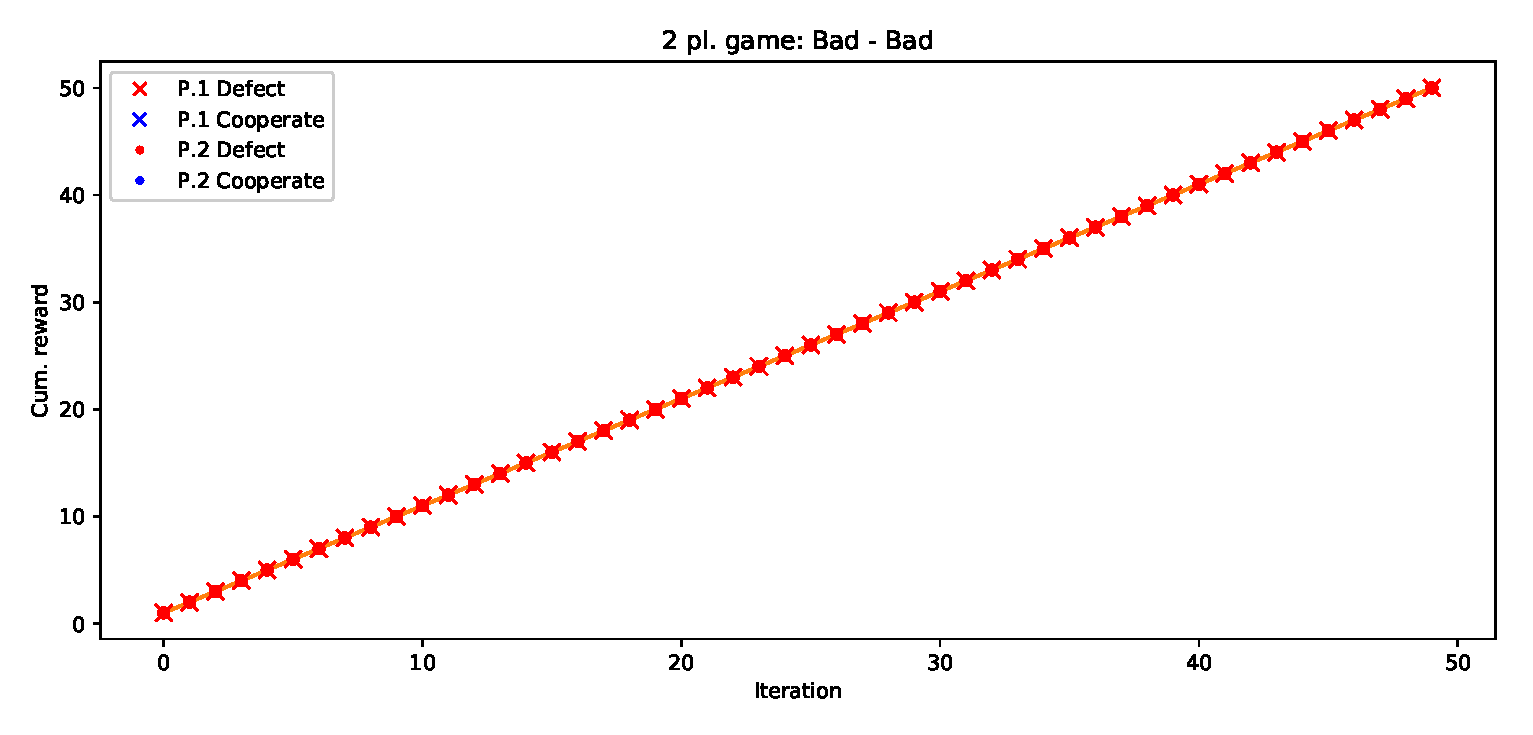
\includegraphics[width=1\columnwidth]{../img/ipd2p/ipd2p-rewards-Bad-Bad}
    \caption{Bad vs Bad}
    \label{fig:badvsbad}
\end{figure}

\begin{figure}[ht]
    \centering
    \includegraphics[width=1\columnwidth]{../img/ipd2p/ipd2p-rewards-Bad-Indifferent.eps}
    \caption{Bad vs Indifferent}
    \label{fig:badvsindiff}
\end{figure}

\begin{figure}[ht]
    \centering
    \includegraphics[width=1\columnwidth]{../img/ipd2p/ipd2p-rewards-Bad-TitForTat}
    \caption{Bad vs TfT}
    \label{fig:badvstft}
\end{figure}

\begin{figure}[ht]
    \centering
    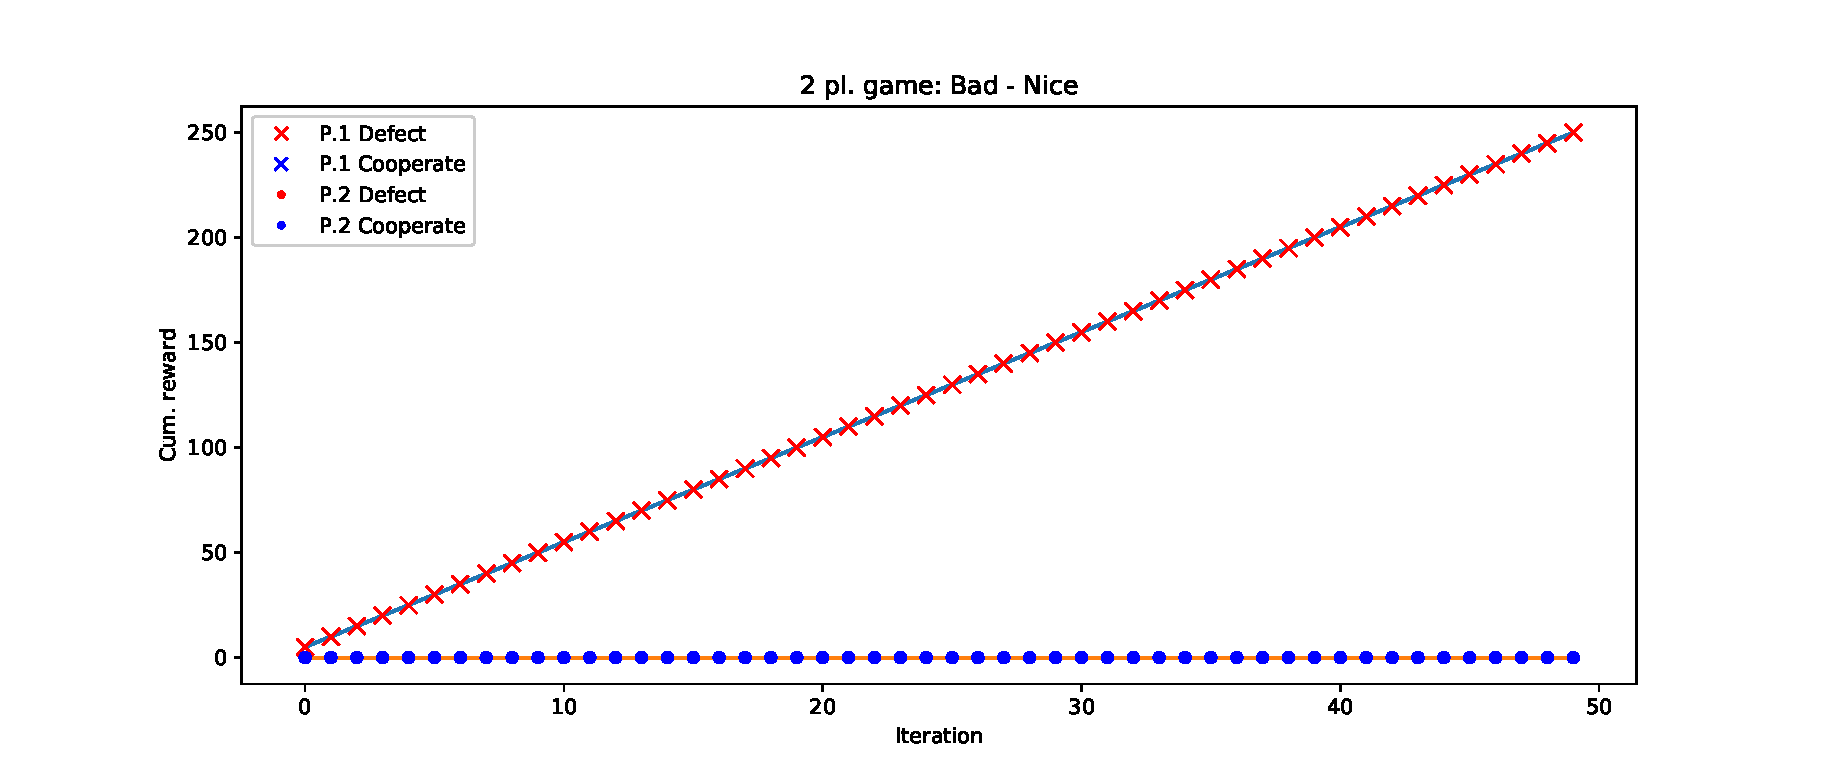
\includegraphics[width=1\columnwidth]{../img/ipd2p/ipd2p-rewards-Bad-Nice}
    \caption{Bad vs Nice}
    \label{fig:badvsnice}
\end{figure}

\begin{figure}[ht]
    \centering
    \includegraphics[width=1\columnwidth]{../img/ipd2p/ipd2p-rewards-Bad-MainlyNice(k=27)}
    \caption{Bad vs Mainly nice}
    \label{fig:badvsmainlynice}
\end{figure}

\begin{figure}[ht]
    \centering
    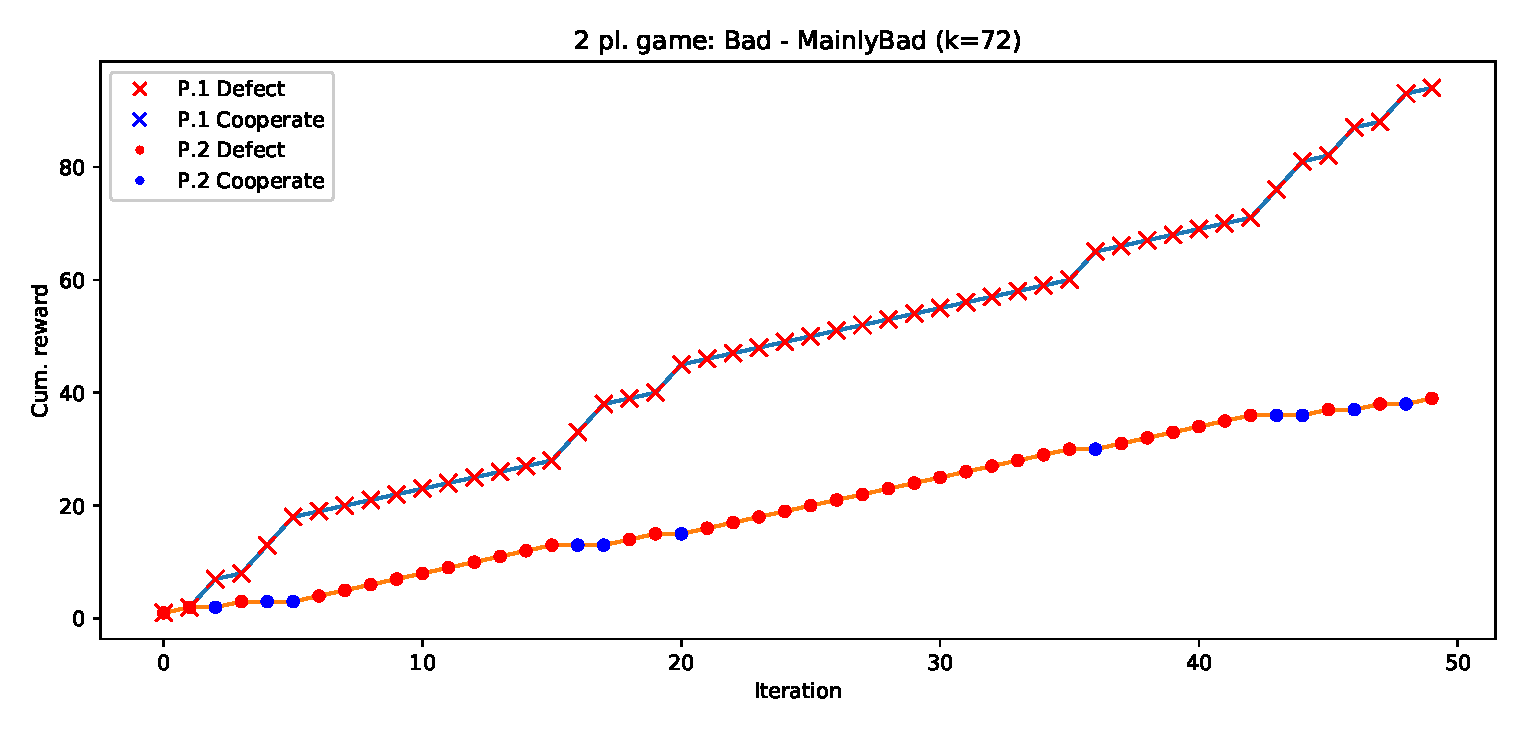
\includegraphics[width=1\columnwidth]{../img/ipd2p/ipd2p-rewards-Bad-MainlyBad(k=72)}
    \caption{Bad vs Mainly bad}
    \label{fig:badvsmainlybad}
\end{figure}

In fact, players might consider a different combination of strategies if they both want to get the highest reward possible: Indifferent-Indifferent, Indifferent-TfT, Nice-Nice or Nice-TfT, TfT-TfT as in Figures~[\ref{fig:indiffvsindiff}, \ref{fig:tftvsindiff}, \ref{fig:nicevsnice}, \ref{fig:nicevstft}, \ref{fig:tftvstft}]. The concept is both player getting the highest reward, not just one of them, in that case it would be the Bad-Nice combination.

\begin{figure}[ht]
    \centering
    \includegraphics[width=1\columnwidth]{../img/ipd2p/ipd2p-rewards-Indifferent-Indifferent}
    \caption{Indifferent vs Indifferent}
    \label{fig:indiffvsindiff}
\end{figure}

\begin{figure}[ht]
    \centering
    \includegraphics[width=1\columnwidth]{../img/ipd2p/ipd2p-rewards-Indifferent-TitForTat}
    \caption{TfT vs Indifferent}
    \label{fig:tftvsindiff}
\end{figure}

\begin{figure}[ht]
    \centering
    \includegraphics[width=1\columnwidth]{../img/ipd2p/ipd2p-rewards-Nice-Nice}
    \caption{Nice vs Nice}
    \label{fig:nicevsnice}
\end{figure}

\begin{figure}[ht]
    \centering
    \includegraphics[width=1\columnwidth]{../img/ipd2p/ipd2p-rewards-TitForTat-Nice}
    \caption{Nice vs TfT}
    \label{fig:nicevstft}
\end{figure}

\begin{figure}[ht]
    \centering
    \includegraphics[width=1\columnwidth]{../img/ipd2p/ipd2p-rewards-TitForTat-TitForTat}
    \caption{TfT vs TfT}
    \label{fig:tftvstft}
\end{figure}

The TfT strategy is interesting, because TfT leads to almost the same cumulative reward as the opponent.
However it might be lower than one in some points \FR{Lower to \emph{what} one?}, since it replicates the previous opponent's move and not the actual move.
A player might choose this move if he/she wants almost the same reward as the opponent.

\textbf{REPETITION}

In conclusion, if a player wants to be sure to win over the other he/she should chose a \textit{Bad guy} strategy, if he/she wants to cooperate as much as possible he/she might choose \textit{TfT, Nice guy} or \textit{indifferent} hoping the opponent chooses one of the strategies in this group.     

In addition to this considerations we have run the simulation multiple times to get insight of mean and variances that rule these games. Obviously the static strategies, or the non-triggering ones, or the the ones without variation have constant mean and $0$ std. What is interesting though is for the random ones as we can see that the results can vary quite a bit.
\textbf{insert images}

If you want to have more insights about this part, the complete collection of the generated pictures can be found in the repository.


\section{Multiple players IPD - Round-robin scheme} \label{s:IPDMP}
In this section an IPD between multiple players (MPIPD) is discussed.
The \textit{round-robin} (RR) scheme, used to match-up the opponents, consists in each player playing once against each As a consequence, the number of players $n = 10$ determines the total number of matches played in the tournament, which in this case is ${n \times (n-1)}/{2} = 45$.
Each player chooses its fixed strategy at the beginning of the tournament and holds it throughout the course of the whole procedure.
As in 2-players IPD, it is possible to set the number of iterations of each match (i.e. \texttt{NUM\_ITER = 50}).

\FR{Below part needs to be adapted to current code}
\EB{IT DEPENDS ON THE INITIAL POPULATION}
We propose a strategy, similar to \textit{Serie A} to assign points to each player after the outcome of the match is determined. A player gets 3 points if he/she wins, 1 point for a draw and 0 points for a loss. A player wins if he/she has a higher reward than the opponent's at the $50-th$ last iteration. He/She looses if the reward is lower and draws if it's the same as the opponent's.
The culumative points after each match are shown in \autoref{fig:mpipd}.
In \autoref{tab:ranking_df} the ranking of the torunament is determined. It can be evaluated that the three players using a \textit{Bad guy} strategy win the tournament.
The strategies can be sorted by most number of points as follows: \textit{Bad guy}, \textit{Mainly bad guy}, \textit{Indifferent}, \textit{Mainly Nice}, \textit{TitForTat} and \textit{Nice}.

The outcome of each match of the tournament can be seen in \autoref{tab:match_df}. \FR{table placeholder here}

\section{Repeated multiple players IPD - RR scheme} \label{s:rIPDMP}
We then used the previuosly defined MPIPD round-robin scheme tournament, iterating it many times to collect more advanced statistics.
We identify this as a \textit{Repeated multiple players IPD} (rMPIPD).
At each tournament repetition, the population is increased adding players with strategies that depend on the results achieved in the previous iteration.

%In our case the population is increasing by one individual that uses the strategy of the previous tournament's winner.
\LA{complete text based on teacher's answer}


\section{Changing rMPIPD - RR scheme} \label{s:crIPDMP}
We introduced mutability in players' strategies when testing the rMPIPD presented above.
Strategies are allowed to mutate \FR{need to say how why and then}.
The gene, a parameter, encodes the attitude of an individual to cooperate. This gene mutates randomly to choose a different strategy at each iteration. The phenotype, which is the strategy, corresponding to that gene competes in the MPIPD such that the best-fitted, which is the winner of the tournament, is determined.

The goal of this task is to simulate the effect of genetic mutations and the effect of natural selection.

In \autoref{fig:cmpipd1} all the players change strategy at each iteration when competing against other players. \textit{Player 7} wins the tournament and the ranking is shown in \autoref{fig:cmpipd1}.

\LA{complete based on teacher's answer}


\section{Conclusion} \label{s:conc}

\FR{Mention the results shall be comparable with the paper.}

\balance
%\bibliographystyle{IEEEtran}
%\bibliography{report}
\end{document}
